Laser Harp consists of four layers. The first layer is the power system, which is going to act as a power source for the device and consists of battery or similar power source. Second layer is frames and components which consists of laser beams, receptors, mister and speaker. Receptors are going to identify the interference in the laser beam and send the signal towards MIDI converter. Mister is being used for visibility whereas speakers are for audio output. Then, we have MIDI converter which is going to receive signals from the receptors and encode those signals as MIDI signals. Finally, the last layer is the sound module which is going to decode the MIDI signals, pass the resulting outcome to fluid synth which in turn sends the audio signals to speakers via sound card. 

\begin{figure}[h!]
	\centering
 	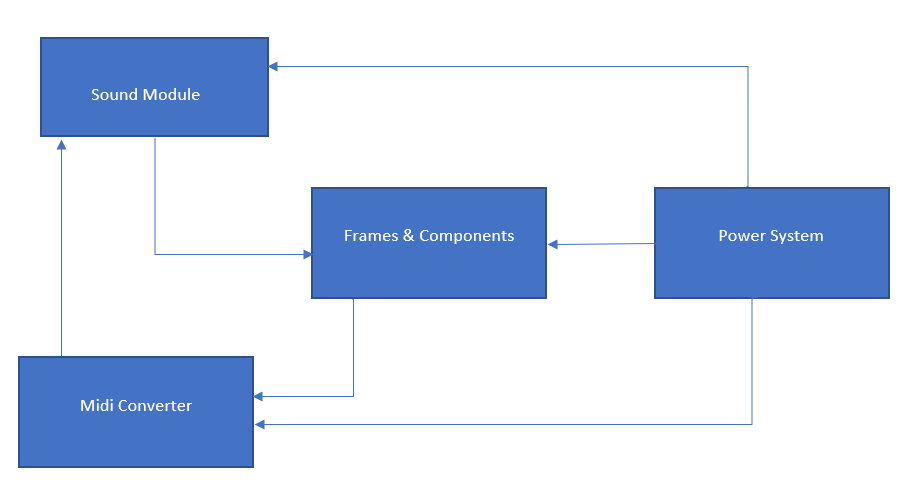
\includegraphics[width=0.60\textwidth]{images/layers}
 \caption{Laser Harp Architectural Layer Diagram}
\end{figure}

\subsection{Power System}
The power system consists of a single component, Battery. It is going to act as a power source for the whole device. The power source would most likely be single or combination of 12V DC 2A batteries.


\subsection{Frames and Components}
Users of the laser harp are going to interact with device using this layer. This layer is going to provide the users with visual and audio output in addition to ways to play the instrument. It consists of laser and receptors, mister and speakers. Lasers acts as both output as well as input medium in the device. Receptors are going to identify the break in the laser beams and transmit the resulting signal towards MIDI converter to be encoded. Lasers are not visible in broad daylight, so  in order to overcome that mister is being used for visibility and is lodged at the base of the harp. Speakers are the way audience are going to hear the resulting audio. It will receive input from sound card form the sound module layer. It will be high quality speaker, able to play multiple range of audio clearly.

\subsection{Sound Module}
This layer is associated with reading the MIDI signals and converting it into audio signals required for the speaker to give out proper audio output. This consists of three subsystems MIDI decoder, fluid synth and sound card. MIDI decoder changes the signals from the MIDI encoder and passes it on to fluid synth. Fluid synth which is enclosed in the raspberry pie is a software that allows the user to control speed, frequency and other characteristics of sound to be produced. Sound card comprises of drivers that enable the raspberry pie to generate audio output.

\subsection{MIDI converter}
This layer is connected to the receptors of the frame and components layer. The interference signal caught by those receptors is changed into MIDI signal by MIDI encoder subsystem lodged in the layer. It is will housed inside a teensy micro controller or the raspberry pie.